% !TEX encoding = UTF-8 Unicode
%!TEX root = memoria.tex
% !TEX spellcheck = es-ES
%%=========================================
\chapter{Metodología}

%%=========================================
\section{Visualización y selección de imágenes}
%%=========================================
\section{Preprocesado}
\subsection{Transformación de formato}

\subsection{Pipeline de preprocesado}

%Imágen de la gráfica simple del pipeline 
El pipeline de preprocesado implementado se compone de las siguientes fases

\begin{enumerate}
\item Selección de volumenes para el procesado
\item Extracción del cerebro del volumen anatómico
\item Slice Timming Correction
\item Corrección del movimiento 
%Imagen plots rotación y traslación
\item Co-registro en dos fases
%Imagen overlap del registro a dos fases 
\item Eliminación de artefactos
\item Band pass filter
\item Suavizado Del inglés \textit{smooth}
%Imagen pre suavizado, kernel 4 y kernel 5 
\end{enumerate}

En la siguiente \ref{preproc:pipeline} se representa gráficamente las distintas fases del preprocesado que se han implementado como primera etapa del presente trabajo.

\begin{figure}[H]
	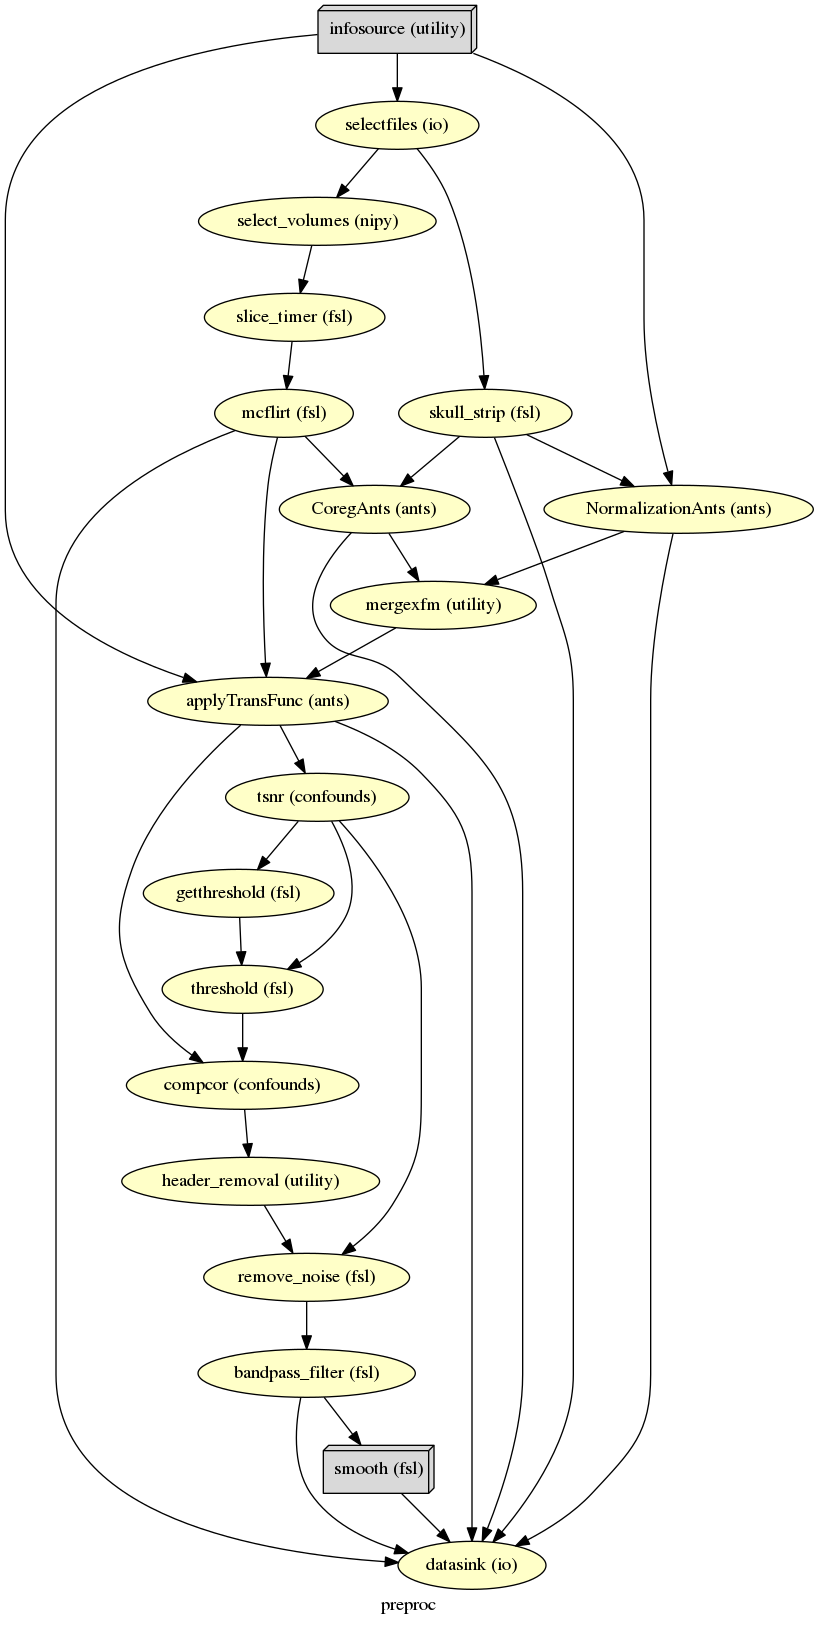
\includegraphics[width=\linewidth, height=\textheight, keepaspectratio]{img/preproc/graph.png}
	\caption{DAG correspondiente con el pipeline de preprocesado}
	\label{preproc:pipeline}
\end{figure}
%%=========================================
\section{Construcción del mapa funcional}

La construcción del mapa funcional se basa en el análisis \hyperref[glos:ica]{ICA}. ICA es un algoritmo de separación de fuente ciega que transforma
un conjunto de señales en sus fuentes latentes asociadas. ICA hace no asumen ningún conocimiento a priori de estas fuentes. La única restricción impuesta a a las fuentes es que son estadísticamente independiente y como mucho uno de ellos es gaussiano.\cite{ica}.

En 1998 aparece el primer metodo de generación de mapas de activación basado en ICA \cite{fmriica}. Elresultado de aplicar ICA a un conjunto de datos 4D, como es el caso del fMRI, es componentes espaciales independientes, cada una de ella correspondiente con su perfil temporal.


Existen varios algoritmos ICA entre los que está el más utilizado \textbf{FastICA}, es un algoritmo de punto fijo que usa la negentropía como función de coste. Tipicamente ICA no se utiliza cn el fin de reducir la dimensionalidad si no para separar las señales superpuestas.



%Analizar la influencia del suavizado sobre la generación del mapa funcional con los dos algoritmos, dictlearn & canICA
Retomando lo comentado en el capítulo 2, el suavivado permite identificar los cambios a mayor escala cuanto mayor es el kernel utilizado ya que estos se ven más evidentes. En la siguiente secuencia de imágenes se puede apreciar la relación de como afecta en el número de regiones encontradas y el tamaño de estás a medida que aumenta el tamaño del diametro del Kernel utilizado.

\begin{figure}[H]
  \begin{subfigure}{\linewidth}
  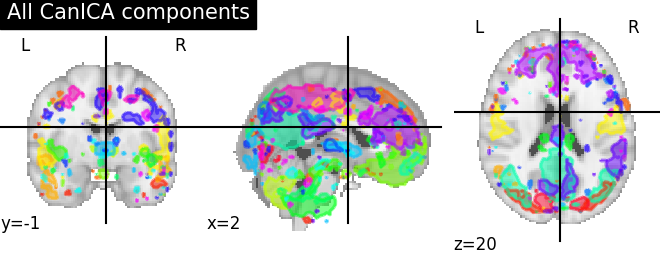
\includegraphics[width=.3\linewidth]{img/canica/canica_None.png}\hfill
  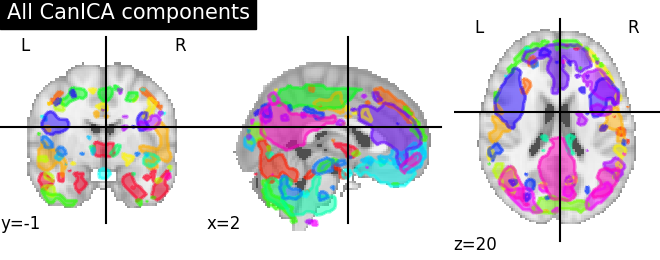
\includegraphics[width=.3\linewidth]{img/canica/canica_4.png}\hfill
  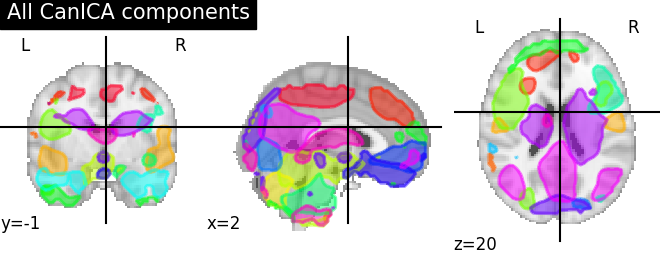
\includegraphics[width=.3\linewidth]{img/canica/canica_8.png}
  \caption{Mapa funcional usando el algoritmo  CanICA con los parámetros de suavizado: None-4mm-8mm}
  \end{subfigure}\par\medskip
  \begin{subfigure}{\linewidth}
  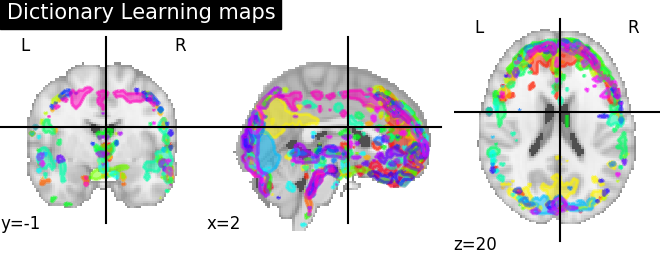
\includegraphics[width=.3\linewidth]{img/canica/dictlearn_None}\hfill
  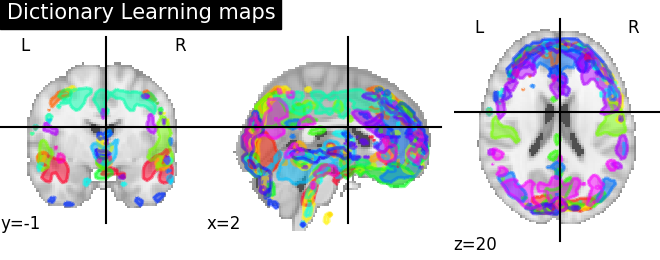
\includegraphics[width=.3\linewidth]{img/canica/dictlearn_4}\hfill
  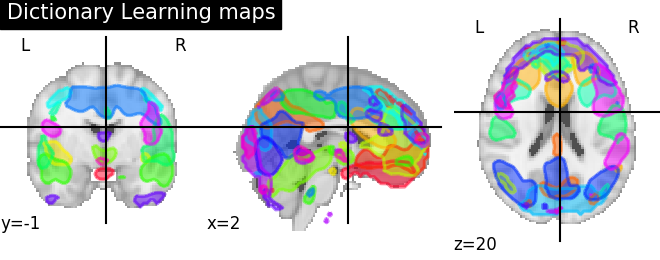
\includegraphics[width=.3\linewidth]{img/canica/dictlearn_8}
  \caption{Mapa funcional usando el algoritmo  DictLearning con los parámetros de suavizado: None-4mm-8mm}
  \end{subfigure}\par\medskip
  \caption{Resultados de diferentes ejecuciones aplicando valores diferentes de suavizado con distintos algoritmos de extracción de mapa funcional}
  \label{preproc:mapa}
\end{figure}

Inicialmente se construye un único mapa de conectividad incluyendo todos los individuos en la misma ejecución. Sin embargo esto no es correcto dado que el experimento asume que la actividad neuronal en reposo de los individuos que padecen de ET, no sigue los mismos patrones de activación que los individuos controles se procede a construir un mapa funcional para cada subconjunto de sujetos. Uno con todos los sujetos que padecen de ET y por tanto se obtendrá un mapa funcional asociado a los patrones de actividad neuronal influenciada por la enfermedad, y otro para los controles que deberían considerarse poseen una actividad \textit{``normal''} y por tanto los patrones de activación deberían aparecer distintos.
 
%%=========================================
\section{Extracción de las regiones y estudio de la conectividad}

\begin{figure}[H]
	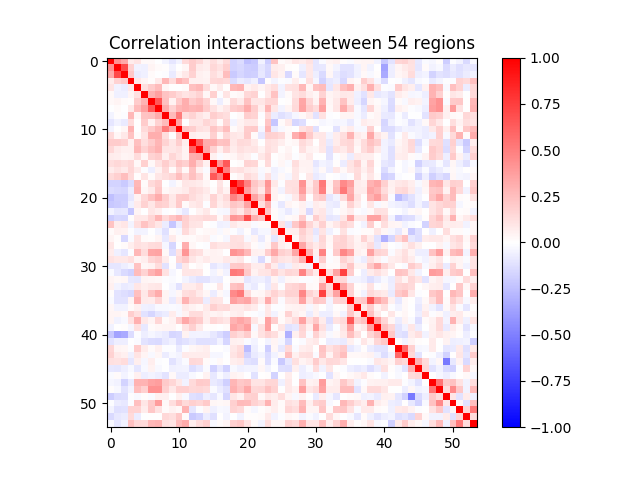
\includegraphics[width=\linewidth, height=\textheight, keepaspectratio]{img/conectividad/matrix.png}
	\caption{Matriz de conecctividad}
	\label{preproc:conectividad}
\end{figure}
%%=========================================
\section{Extracción de parámetros}
\subsection{Entropía Espectral de Shannon}
%Gráfica
\subsubsection{Espectro de potencia}
%Gráfica
\subsection{Entropía de permutación}
%Gráfica
%%=========================================

